\documentclass[11pt]{article}

% Packages
\usepackage{amsmath}
\usepackage{graphicx}
\usepackage{amssymb}
\usepackage{longtable}
\usepackage[spanish]{babel}
\usepackage[utf8]{inputenc}
\usepackage[T1]{fontenc}
\usepackage{float}


\author{Brian Ameht Inclán Quesada C-411\\ Davier Sánchez Bello C-412\\ Eric López Tornas C-411}
\title{Proyecto Final de IA y Simulación \\ Juego de Supervivencia}
\date{}

% Document
\begin{document}

\maketitle
\newpage

\tableofcontents
\newpage

\section{Introducción}

\section{Modelo}
\subsection{Resumen del modelo}
\subsection{Ventajas}
\subsection{Desventajas}
\subsection{Posibles mejoras}


\section{Implementación}
\subsection{Modelo de la simulación}
\subsection{Agentes}
\subsection{Base de conocimiento y toma de decisiones}
Este sistema se basa en una estructura modular que integra hechos y reglas dentro de un motor de inferencia para gestionar y tomar decisiones basado en conocimientos. Está diseñado para funcionar en entornos donde las decisiones se toman a partir de un conjunto de datos dinámico y posiblemente en tiempo real. Los componentes clave son:

\begin{itemize}
    \item \textbf{Enumeración \textit{Knowledge}:} Es una enumeración que define diferentes tipos de conocimientos que pueden ser importantes en un contexto de toma de decisiones. Estos incluyen aspectos como la posición, la salud, los ataques disponibles, las asociaciones y más. Cada tipo de conocimiento sirve como una clave que identifica un tipo de información específica dentro del sistema
    \item \textbf{Clase \textit{Fact}:}  Representa un hecho o una pieza de información en el sistema. Cada hecho está compuesto por una clave (un valor de Knowledge) y un dato asociado a esta clave. Esta estructura permite almacenar y gestionar información dinámica que el sistema utiliza para tomar decisiones
    \item \textbf{Clase \textit{Rule}:}  Define una regla en el sistema, la cual consta de una condición y una acción. La condición es una función que toma un conjunto de hechos y determina si la regla debe ejecutarse. Si la condición es verdadera, la acción (también una función) se ejecuta para generar nuevos hechos basados en los hechos existentes. En resumen, esta clase permite definir la lógica del sistema para generar nuevos hechos a partir de los existentes.
    \item \textbf{Clase \textit{BaseKnowledge}:} Esta clase especifica las operaciones fundamentales para cualquier sistema de conocimiento, como aprender y tomar decisiones.
    \item \textbf{Clase \textit{Estrategy}:} Es una implementación concreta de BaseKnowledge. Gestiona un conjunto de hechos y reglas a través de un motor de inferencia. Permite añadir y eliminar conocimientos y reglas, aprender de nuevos datos y tomar decisiones basadas en las reglas definidas y los hechos actuales
    \item \textbf{Clase \textit{InferenceEngine}:} Es el componente que realiza la inferencia lógica. Gestiona un conjunto de hechos y reglas, permitiendo añadir y eliminar estos elementos. El método run de InferenceEngine es crucial: evalúa todas las reglas con los hechos actuales para generar nuevos hechos, los cuales pueden influir en decisiones futuras.
\end{itemize}

Este modelo permite un manejo flexible y dinámico de información, esencial para la toma de decisiones en entornos cambiantes, tal y como necesitamos en nuestra simulacion.
\subsection{Algoritmos de búsqueda}
En esta sección, describiremos varios algoritmos de búsqueda utilizados en nuestro proyecto. Cada algoritmo será tratado en una subsección independiente, donde se explicará su funcionamiento, particularidades y ejemplos de uso.

\subsubsection{Algoritmo A*}
El algoritmo A* es una técnica de búsqueda de camino que encuentra el camino más corto entre un nodo inicial y un nodo objetivo en un grafo. Utiliza una combinación de costos conocidos para llegar a un nodo \( g(n) \) y una estimación heurística \( h(n) \) del costo para alcanzar el objetivo desde ese nodo. La función \( f(n) = g(n) + h(n) \) guía el algoritmo para explorar los caminos más prometedores primero.

En nuestro caso estamos implementado usando una estructura de tipo $min-heap$, denominada $open\_heap$. Esta estructura se utiliza para mantener los nodos que aún necesitan ser explorados en el algoritmo. Mediante un heap de minimos organiza los elementos de tal manera que el primer elemento es siempre el más pequeño, lo cual es útil para extraer rápidamente el nodo con el costo estimado más bajo para continuar la búsqueda.


\paragraph{Detalles del Funcionamiento}
\begin{itemize}
    \item \textbf{Heurística}: La función heurística es crucial en A*. Una elección común es la distancia Manhattan, útil en grillas donde solo se permiten movimientos horizontales y verticales.
    \item \textbf{Conjunto de abiertos}: A* mantiene un conjunto de nodos conocidos como el "conjunto abierto". Inicialmente, contiene solo el nodo de inicio.
    \item \textbf{Bucle Principal}: En cada paso del algoritmo, el nodo con el menor valor de \( f(n) \) se retira del conjunto abierto. Este nodo es procesado considerando todos sus nodos vecinos. Para cada vecino, se calcula \( g(n) \) y \( h(n) \), y si el nuevo camino es mejor, se actualiza el camino.
\end{itemize}

\paragraph{Ejemplo de Uso}
En el siguiente ejemplo mostramos un agente del tipo $FoodSeekerAgent$ que en nuestra simulacion representa al agente que esta constantemente buscando la mejor manera de llegar al lugar donde mas recursoa halla. En este caso tenemos un tablero de \(10 \times 10\). Definimos la posición inicial como \( (0, 8) \) y el objetivo en este caso la casilla que dentro de su rango de vision
es la que mas recursos posee, como \( (2, 9) \). La salida del algoritmo proporcionará la secuencia de movimientos para llegar del inicio al objetivo, evitando los obstáculos, que en este ejemplo no hay ninguno.

\begin{figure}[H]
    \centering
    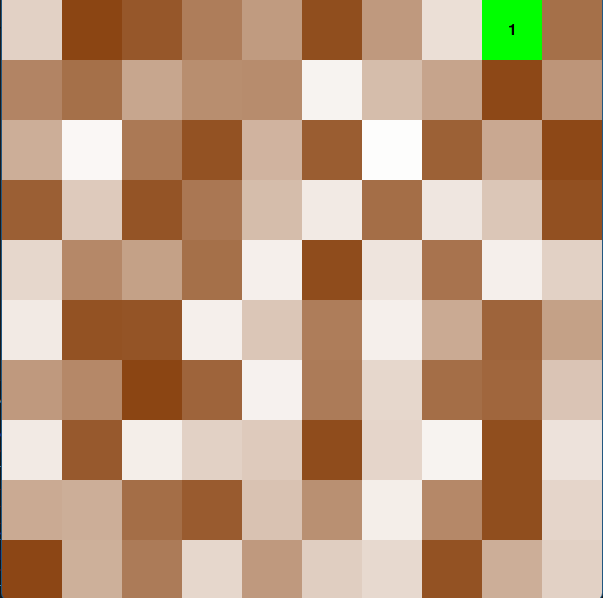
\includegraphics[width=0.18\textwidth]{images/image1.png}\hfill
    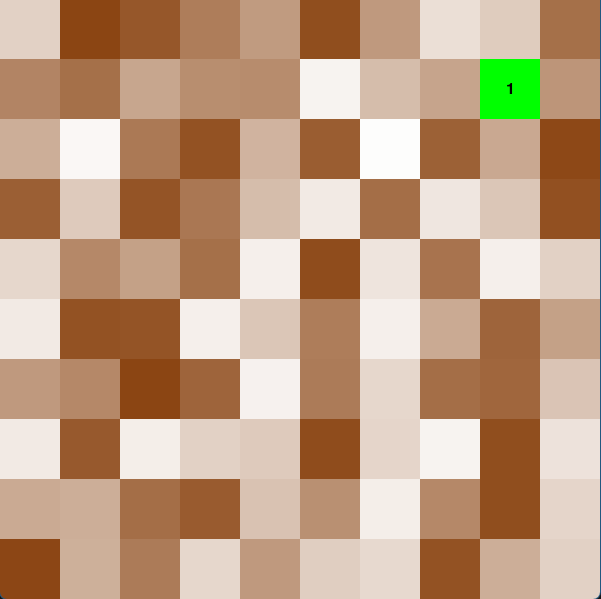
\includegraphics[width=0.18\textwidth]{images/image2.png}\hfill
    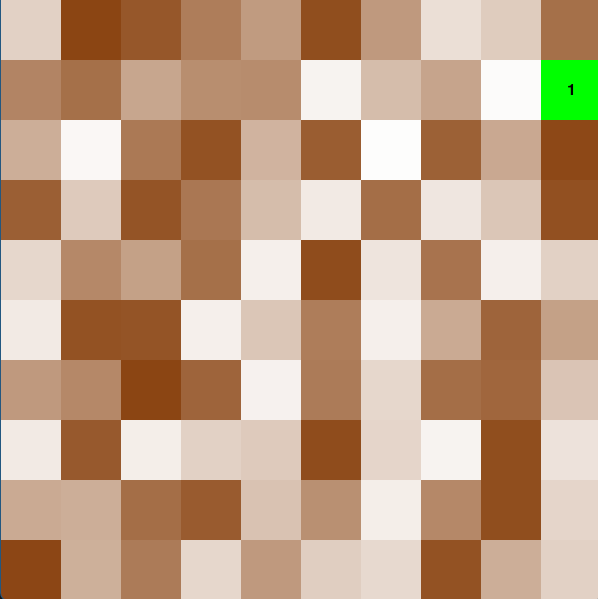
\includegraphics[width=0.18\textwidth]{images/image3.png}\hfill
    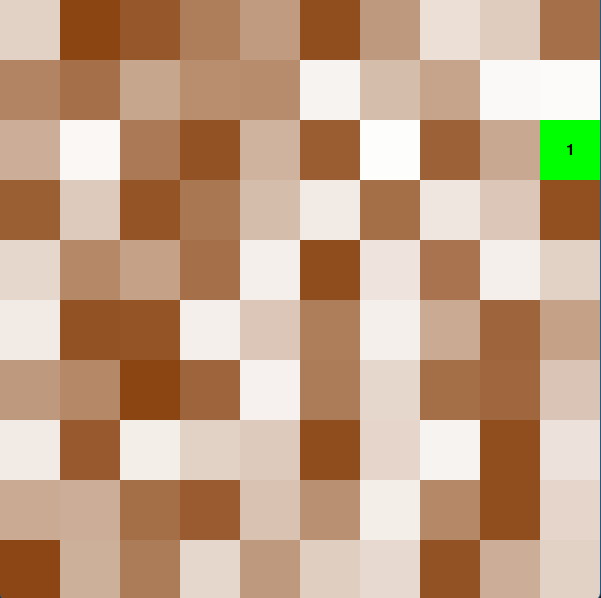
\includegraphics[width=0.18\textwidth]{images/image4.png}
    \caption{Secuencia de movimientos del agente FoodSeekerAgent en la simulación desde la posicion \( (0, 8) \) hasta \( (2, 9) \) .}
\end{figure}

\paragraph{Implementación}
Para implementar el A* en la simulación de nuestro juego, utilizamos una clase que gestiona la verificación de movimientos válidos y obstáculos. Esta clase ajusta el algoritmo para adaptarse a las características específicas del entorno de juego, como áreas inaccesibles y diferentes costos de movimiento asociados con diversos tipos de terreno.

\subsubsection{Búsqueda en Amplitud (BFS)}
La Búsqueda en Amplitud, o BFS por sus siglas en inglés (Breadth-First Search), es un algoritmo clásico para explorar grafos y árboles. Es especialmente útil en situaciones donde necesitamos encontrar el camino más corto en términos de número de aristas entre un nodo de origen y otros nodos, dado que explora todos los nodos a la misma profundidad antes de moverse a la profundidad siguiente.
En nuestra simulación está especialmente diseñado para calcular rutas de escape en situaciones donde un agente necesita maximizar la distancia de un atacante en un entorno de grilla. La adaptación permite a los usuarios elegir entre obtener sólo el siguiente movimiento óptimo o el camino completo de escape.

\paragraph{Funcionamiento de BFS}
La implementación de BFS comienza con la inserción del nodo de origen en una cola. A medida que cada nodo se procesa, sus vecinos no visitados se añaden al final de la cola. Este proceso continúa hasta que se visitan todos los nodos alcanzables o hasta que se encuentra el nodo objetivo, lo que permite una exploración completa en capas.

\begin{itemize}
    \item \textbf{Cola de BFS}: Utilizamos una cola para mantener el orden de exploración de los nodos. En nuestra implementación, esto se maneja con una estructura de datos deque para una eficiente inserción y eliminación de elementos.
    \item \textbf{Conjunto de Obstáculos y Visitados}: Mantenemos un conjunto de obstáculos para evitar la exploración de nodos no transitables y un conjunto de nodos visitados para evitar procesar el mismo nodo más de una vez.
    \item \textbf{Validación de Movimientos}: Cada movimiento potencial se valida para asegurar que no se salga del límite del entorno de juego y no se encuentre con obstáculos.
\end{itemize}

\paragraph{Ejemplo de Uso}
En el siguiente ejemplo, mostramos un agente del tipo $PacifistAgent$ en la posicion \( (5, 6) \), que en nuestra simulación representa al agente que tiene una estrategia pacifica, evade los ataques e intenta sobrevivir.
En este caso, tenemos un tablero de \(7 \times 7\). Definimos la posición inicial del agente $CombatantAgent$ como \( (3, 3) \). La salida del algoritmo proporcionará la secuencia de movimientos para llegar a la posición segura más lejana posible, evitando al atacante, evidenciamos en las siguientes imagenes como
la secuencia de movimientos incluye como primer movimiento el de alejarce del atacante hacia la casilla \( (6, 6) \), luego en el siguiente movimiento, este se queda en esa misma posicion ya que de entre las posibles es la mas lejana al atacante


\begin{figure}[H]
    \centering
    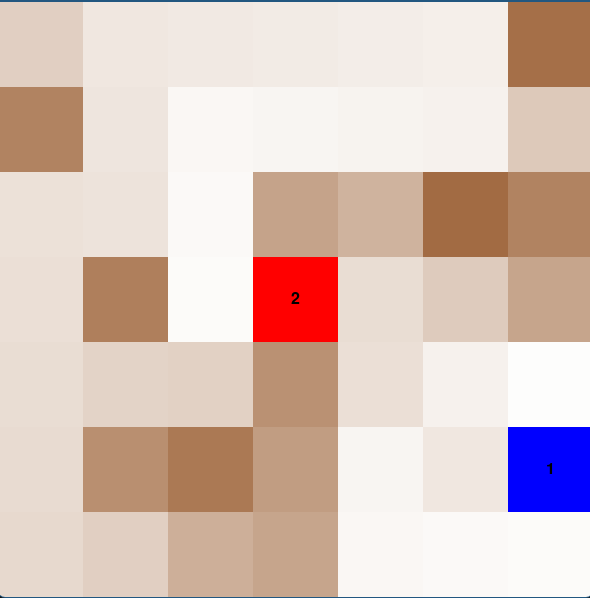
\includegraphics[width=0.18\textwidth]{images/image6.png}\hfill
    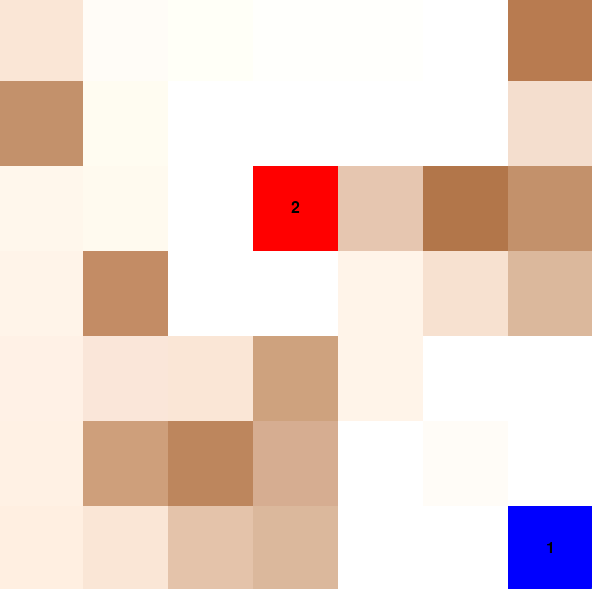
\includegraphics[width=0.18\textwidth]{images/image7.png}\hfill
    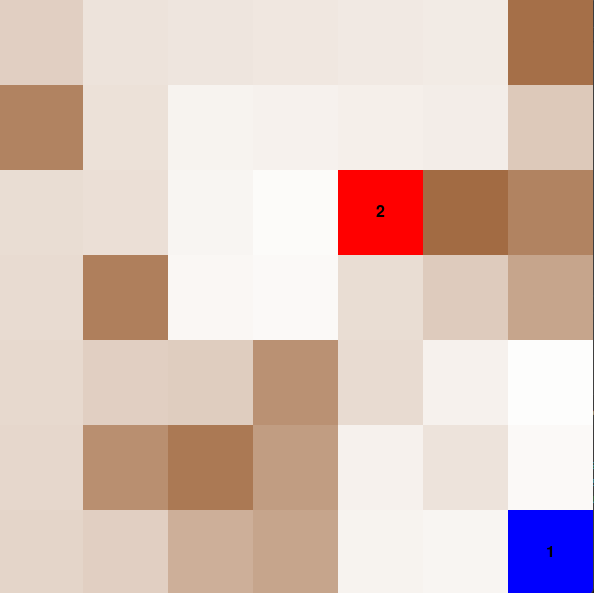
\includegraphics[width=0.18\textwidth]{images/image8.png}
    \caption{Secuencia de movimientos calculada por BFS para evadir al atacante, mostrando cada paso desde el inicio hasta la posición segura más lejana posible.}
\end{figure}

\paragraph{Implementación}
Nuestra clase \textit{BFS} incluye métodos para configurar los obstáculos y calcular la ruta basada en las posiciones dinámicas de los agentes y las barreras en el entorno. Esto asegura que el agente siempre tenga una ruta de escape actualizada y pueda reaccionar a los cambios en el entorno.



\subsubsection{Monte Carlo Tree Search (MCTS)}
El Monte Carlo Tree Search es un algoritmo de búsqueda heurística utilizado para la toma de decisiones en juegos de perfecta información. Combina la exploración aleatoria de árboles con la simulación para evaluar los movimientos potenciales.

\paragraph{Funcionamiento y Ejemplos}
Descripción del funcionamiento y ejemplos...



\subsection{LLM}
Utilizamos el LLM para la creación de agentes y la configuración del escenario de la simulación, así como para la función de comentarista del juego. Para la creación de agentes, empleamos una lista con descripciones por defecto de los comportamientos de nuestros tipos de personajes y la información suministrada por el usuario. El LLM infiere cuál es el tipo de personaje por defecto que más se acerca a la descripción del usuario, así como las estadísticas, teniendo en cuenta la mención u omisión de aspectos positivos y negativos en la descripción del personaje.
\\
En cuanto a la creación del mapa, se eligen las dimensiones del escenario a simular de acuerdo a la inferencia realizada por el LLM en la descripción del terreno.  \\
Para la función de comentarista, alimentamos al LLM con las últimas acciones ocurridas en la simulación y las descripciones de los personajes. Esto permite al modelo crear un breve relato de los eventos más recientes no comentados en la simulación.
\subsection{Interfaz de la simulación}

\section{Análisis de la simulación}
\section{Conclusiones}

\end{document}
